\chapter{Interest Rate Volatility and Derivatives}\label{chap::LMM}

Before introduction of the market models, short rate models are widely used by practitioners for interest rate derivatives pricing. Examples of short-rate models are \cite{vo97} model, \cite{cir85} model and \cite{jh90} model. These models establish the instantaneous spot interest rate dynamics, using single or multi-dimensional diffusion process(es). However, the interest rate dynamics from short rate models is not compatible with Black's formula for either swap or swaption. In other words, simplified and inexact assumptions are made on interest rate distribution in short rate models, in order to extrapolate the term structure of rates. This knowledge of term structure is vital to interest rate derivatives pricing. The lack of calibration to the whole forward curve is a trade-off with mimicking the Black-Scholes model for stock option in interest rate option, but brings in market inconsistency.

The LIBOR market model (LMM), instead, is based on the discretization of the yield curve into discrete forward rates. And each of these forward rate represents to the market quote of corresponds Forward Rate Agreement (FRA). More importantly, the LIBOR market model prices caps with Black's cap formula (lognormal forward-LIBOR model, LFM) and prices swaption with Black's swaption formula (lognormal forward-swap model, LSM). That is, the interest rate dynamics from the LMM are consistent with caps and swaptions, which are two most standard and basic interest-rate option on the market.

\section{LMM Framework}
\subsection{Forward Rate}
In standard LMM, we assume that the stochastic differential equation of each $n$ spanning forward rates $f_i$ formulates as
\begin{equation} \label{eqn::forward_rate}
\frac{d f_i}{f_i} = \mu_i (\mathbf{f}, t)dt + \sigma_t(t) d\tilde{W_i}
\end{equation}
where $\mathbb{E}[ d\tilde{W_i}  d\tilde{W_j}] = \rho_{ij} dt$. The lognormal-type model setup ensures positive forward rates. And $i,j=1,2,\ldots,M$. The derivative of Black's formula for caplets is detailed in Appendix

\subsection{Numeraire and Measure}
Consider the forward (adjusted) probability measure $Q^i$ associated with numeraire $P(\cdot,T_i)$ for maturity $T_i$, where the price of the bond maturity coincides with the forward rate maturity. With simple compounding, it follows
$$
d f_i P(t,T_i) = [P(t,T_{i-1}) - P(t,T_{i-1})] / \tau_i
$$
Note that $f_i P(t,T_i)$ is a tradable asset's price, where the price divides by the numeraire $P(\cdot,T_i)$ is $f_i(t)$ itself. Therefore, $f_i(t)$ follows a martingale under forward measure. Corresponding driftless dynamics for $f_i(t)$ under this measure with respect to Equation~\ref{eqn::forward_rate} is
$$
\frac{d f_i(t)}{f_i(t)} = \sigma_i(t) dW_i(t)
$$
When $\sigma$ is bounded and using Ito's formula, the unique strong solution of the forward rate dynamic is
$$
\log f_i (T) = \log f_i(0) - \int_0^T \frac{\sigma_i(t)^2}{2} dt + \int_0^T \sigma_i(t) dW_i(t)
$$
The instantaneous volatility term $\sigma_i(t)$ assumes to be piecewise-constant
$$
\sigma_i(t) = \sigma_{i,\beta(t)}(t)
$$
where in general $\beta(t)=m$ if $T_{m-2}<t \leq T_{m-1}, m\geq 1$.

Under this lognormal assumption, it yields that the dynamics of $f_k$ under forward measure $Q^i$ in three cases $i<k, i=k$ and $i>k$ are
\begin{eqnarray*}
i<k,& t\leq T_i: df_k(t) = \sigma_k(t)f_k(t)\sum_{j=i+1}^{k}\frac{\rho_{k,j}\tau_j\sigma_j(t)f_j(t)}{1+\tau_j f_j(t)}dt + \sigma_k(t) f_k(t) dW_k(t) \\
i=k,& t\leq T_{k-1}: df_k(t) = \sigma_k(t) f_k(t) dW_k(t) \\
i>k,& t\leq T_{k-1}: df_k(t) = -\sigma_k(t)f_k(t)\sum_{j=i+1}^{k}\frac{\rho_{k,j}\tau_j\sigma_j(t)f_j(t)}{1+\tau_j f_j(t)}dt + \sigma_k(t) f_k(t) dW_k(t)
\end{eqnarray*}
where $W=W^i$ is a Brownian motion under $Q^i$.

\subsection{Risk Neutral Dynamics in LMM}
According to~\cite{bm06}, the risk-neutral dynamics of forward LIBOR rates in the LMM is
$$
d f_i(t) = \tilde{\mu}_i(t) f_i(t)dt + \sigma_i(t)f_i(t) d \tilde{W}_i(t)
$$
where
\begin{eqnarray*}
\tilde{\mu}_i(t) &=& \sum_{j=\beta(t)}^{i} \frac{\rho_{i,j}\tau_j\sigma_i(t)\sigma_j(t)f_j(t)}{1+\tau_j f_j(t)} + \tilde{\sigma}_i(t)\rho\int_t^{T_{\beta(t)-1}}\tilde{\sigma}_f(t,u)'du \\
                 &=& \sum_{j=\beta(t)}^{i} \frac{\rho_{i,j}\tau_j\sigma_i(t)\sigma_j(t)f_j(t)}{1+\tau_j f_j(t)} + \sum_{j=\beta(t)}^{i} \rho_{i,j}\sigma_i(t)\rho\int_t^{T_{\beta(t)-1}}\tilde{\sigma}_f(t,u)'du
\end{eqnarray*}
where $\tilde{\sigma}$ is the horizontal $M$-vector volatility coefficient for the forward rate $f_i(t)$.


\section{Calibration of LMM to Caps/Swaptions Prices}
Let's assume a unit notional amount, adn the discount payoff at time 0 of a cap with reset date $T_{\alpha}$ and payment dates $T_{\alpha+1},\ldots,T_{\beta}$ is given by
$$
\sum_{i=\alpha+1}^{\beta} \tau_i D(0,T_i)(f(T_{i-1},T_{i-1},T_{i}))^+
$$

The risk neutral expectation on the cap price described above is
$$
\mathbb{E} \left\{ \sum_{i=\alpha+1}^{\beta} \tau_i D(0,T_i)(f(T_{i-1},T_{i-1},T_{i}))^+ \right\} = \sum_{i=\alpha+1}^{\beta} \tau_i P(0,T_i) \mathbb{E}^i[(f(T_{i-1},T_{i-1},T_{i}))^+]
$$

Therefore the caplet (the single additive term) is then given by
$$
P(0,T_i)\mathbb{E}^i(f_i(T_{i-1})-K)^+
$$

According to Proposition 6.4.1 in~\cite{bm06}, the price of the $T_{i-1}$-caplet implied by the LMM coincides with that given by the corresponding Black caplet formula
\begin{eqnarray*}
Cpl^{LMM}(0,T_{i-1},T_i,K)  &=& Cpl^{LMM}(0,T_{i-1},T_i,K,v_i) \\
                            &=& P(0,T_i)\tau_i Bl(K,f_i(0),v_i) \\
            Bl(K,f_i(0),v_i) &=& \mathbb{E}^i (f_i(T_{i-1})-K)^+ \\
                            &=& f_i(0) \Phi(d_1(K,f_i(0), v_i)) - K \Phi(d_2(K,f_i(0), v_i)) \\
            d_{1,2}(K,f,v)  &=& \frac{\log(f/K) \pm v^2/2}{v}
\end{eqnarray*}

The market quote on the market is typically with first reset date in three months or in six months. An equation is considered between the market price $Cap^{MKT}(0,T_i,K)$ of the cap with $\alpha=0$ and $\beta=j$ and the sum of the first $j$ caplets prices:
$$
Cap^{MKT}(0,T_i,K) = \sum_{i=1}^{j} \tau_i P(0,T_i) Bl(K,f_i(0),\sqrt{T_{i-1} v_{T_j-cap}})
$$
where a same average-volatility value $v_{T_j-cap}$ has been put in all caplets up to $j$. To recover the market cap prices with  forward rate dynamics we have
$$
\sum_{i=1}^{j} \tau_i P(0,T_i) Bl(K,f_i(0),\sqrt{T_{i-1} v_{T_j-cap}}) = \sum_{i=1}^{j} \tau_i P(0,T_i) Bl(K,f_i(0),\sqrt{T_{i-1} v_{T_{i-1}-caplet}})
$$

Recovering the $v_{caplet}$'s from the market quoted $v_{cap}$'s using stripping algorithm can be used, which based on the last equality applied to $j=1,2,3,\ldots$.

In this project, I use the swaption normal volatility to calibration the LMM. The swaption is an option whose under is an interest rate swap (IRS). The discounted payoff of an IRS with a K different from swap rate can be expressed as
$$
D(0,T_{\alpha})(S_{\alpha,\beta}(T_{\alpha}-K)\sum_{i=\alpha+1}^{\beta} \tau_i P(T_{\alpha}, T_i))
$$

And a swaption is a contract that gives its buyer the right, but not obligation, to enter a future time an interest rate swap. The payer swaption payoff is
$$
D(0,T_{\alpha})(S_{\alpha,\beta}(T_{\alpha}-K)^+\sum_{i=\alpha+1}^{\beta} \tau_i P(T_{\alpha}, T_i))
$$

The coincidence of payer swaption price with Black's formula for swaptions is addressed in Proposition 6.7.1 in~\cite{bm06}, which states
\begin{eqnarray*}
PS^{LMM}(0,T_{\alpha},[T_{\alpha},\ldots,T_{\beta}],K) &=& PS^{Black}(0,T_{\alpha},[T_{\alpha},\ldots,T_{\beta}],K) \\
            &=& C_{\alpha,\beta}(0)Bl(K,S_{\alpha,\beta}(0),v_{\alpha,\beta}(T_\alpha))
\end{eqnarray*}

The calibration process of swaptions prices to LMM parameters is to keep adjusting the correlation matrix in the LMM so that the difference between market observed volatility is closest to the model generated volatilities. The Rebonato calibration method is detailed in~\cite{re99} and \cite{re02}.

The market date I chose for LMM calibration is 2016-06-30. The U.S. swaption normal volatility date source is Bloomberg. The normal volatilities are from vanilla European swaptions with specific option tenors and swap tenors. Figure~\ref{fig::swaption_normal_vol} plots the market observable swaption normal volatilities with respect to various option terms and swap terms. Note that the volatilities of swaption used for calibration are all at-the-money level volatilities.

\begin{center}
  \begin{figure}
  \centering
      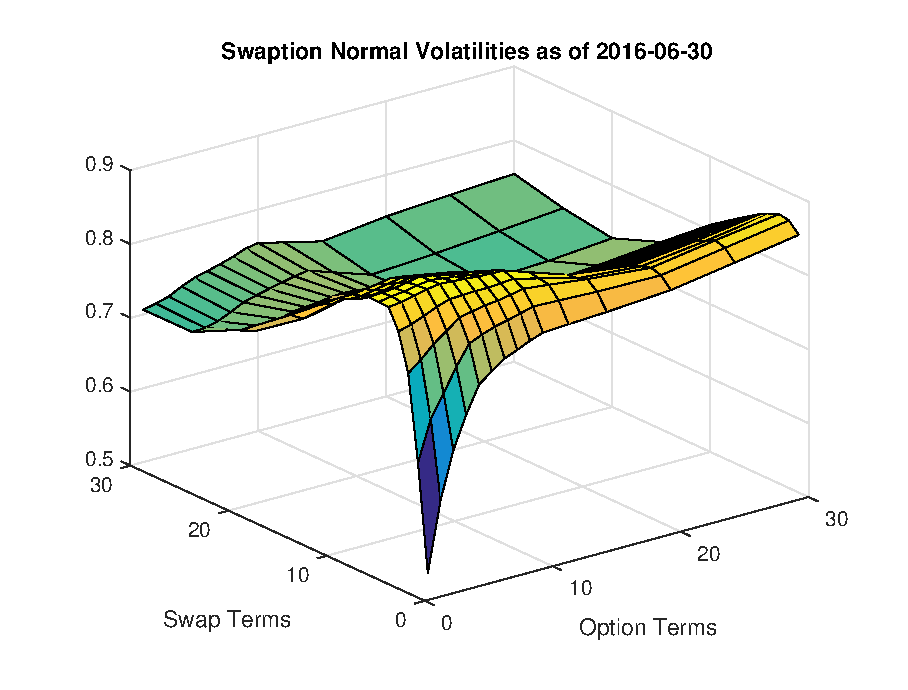
\includegraphics[scale=0.6]{swaption_normal_vol.eps}
      \caption{The normal volatilities of swaptions as of 2016-06-30. Data source is Bloomberg.}\label{fig::swaption_normal_vol}
  \end{figure}
\end{center}

The U.S. LIBOR OIS curve for the same market date is used to discount the payoff of the swaption. The selected discounting method is dual-curve discounting, where the discount factor comes from the OIS curve. Figure~\ref{fig::curves} plots the zero and forward curves as of market date 2016-06-30.

\begin{center}
  \begin{figure}
  \centering
      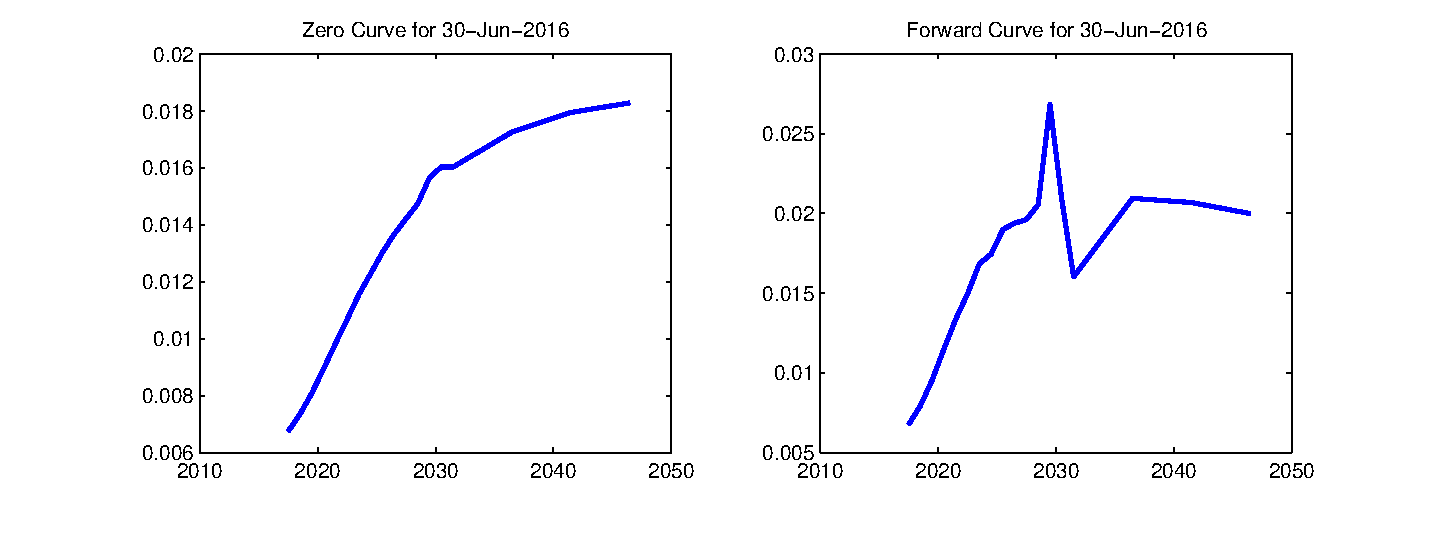
\includegraphics[scale=0.6]{zero_forward_curves.eps}
      \caption{The zero curve (left) and forward curves (right) as of 2016-06-30.}\label{fig::curves}
  \end{figure}
\end{center}

The LMM calibration has objective function that calculates the difference between LMM generated Black volatilities and the market observed Black volatilities. The market observable Black volatilities is backed out from swaption normal volatilities using the Black model. The LMM projected Black volatilities are calculated from tuned LMM parameters and Black's formula for swaption pricing. A set of market consistent parameters, especially the correlation matrix from the LMM, is optimized using least square technique. A least square type of error is minimized between the market volatility surface and LMM projected surface. The calibration process implementation is detailed in the code submitted among with this paper.

The option and swap tenors used for calibration are 1-Yr, 3-Yr, 5-Yr. 7-Yr, 10-Yr, 20-Yr and 30-Yr, in total 49 data points from the volatility surface. The parametric correlation function takes the form $\rho_{i,j}=\exp(-\beta(t)|i-j|)$, and a piecewise constant instantaneous volatility assumption is selected. One useful approximation (Rebonato 2002) follows as below, which computes the Black volatility for a European swaption, given an LMM with a set of volatility functions and a correlation matrix.
$$
(v_{\alpha_\beta}^{LMM})^2 = \sum_{i,j=\alpha+1}^{\beta} \frac{w_{i}(0)w_{j}(0)f_i(0)f_j(0)\rho_{i,j}}{S_{\alpha,\beta}(0)^2} \int_0^{T_{\alpha}} \sigma_i(t)\sigma_j(t) dt
$$
where
$$
w_i(t) = \frac{\tau_i P(t,T_i)}{\sum_{k=\alpha+1}^{\beta} \tau_k P(t,t_k)}
$$

The calibration is achieved via optimization Rebonato method. Figure~\ref{fig::vol_term} plots the term structure of the volatility from the calibrated LMM parameters.

\begin{center}
  \begin{figure}
      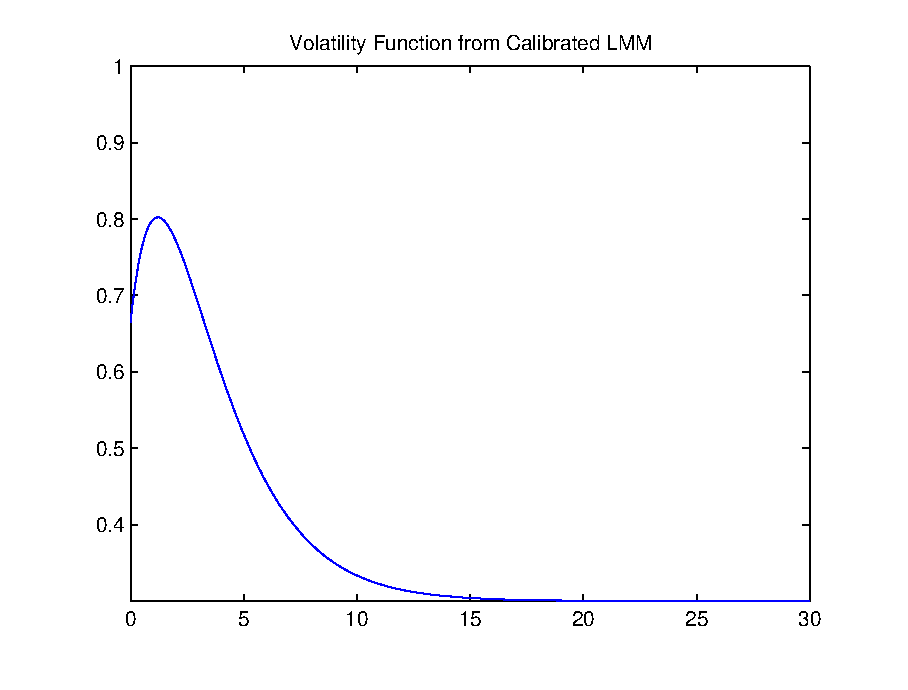
\includegraphics[scale=0.6]{vol_func.eps}
      \caption{The term structure of volatility from calibrated LMM.}\label{fig::vol_term}
  \end{figure}
\end{center}

Another benefit of calibrating market consistent model parameters is to populate market consistent interest rate scenarios for exotic option pricing. In this project, I use the LMM generated scenarios to price vanilla swaption (as discussed in~\ref{chpt::market_risk}) and Bermudans swaption. For a Bermudans swaption with maturity date in 5 years and a strike of 0.045, the averaged price is \$3.250, over 500 scenarios. Figure~\ref{fig::sim_zero_forward} plots the simulated zero curves and forward curves in one scenario (out of 1000) from the calibrated LMM.

\begin{center}
  \begin{figure}
      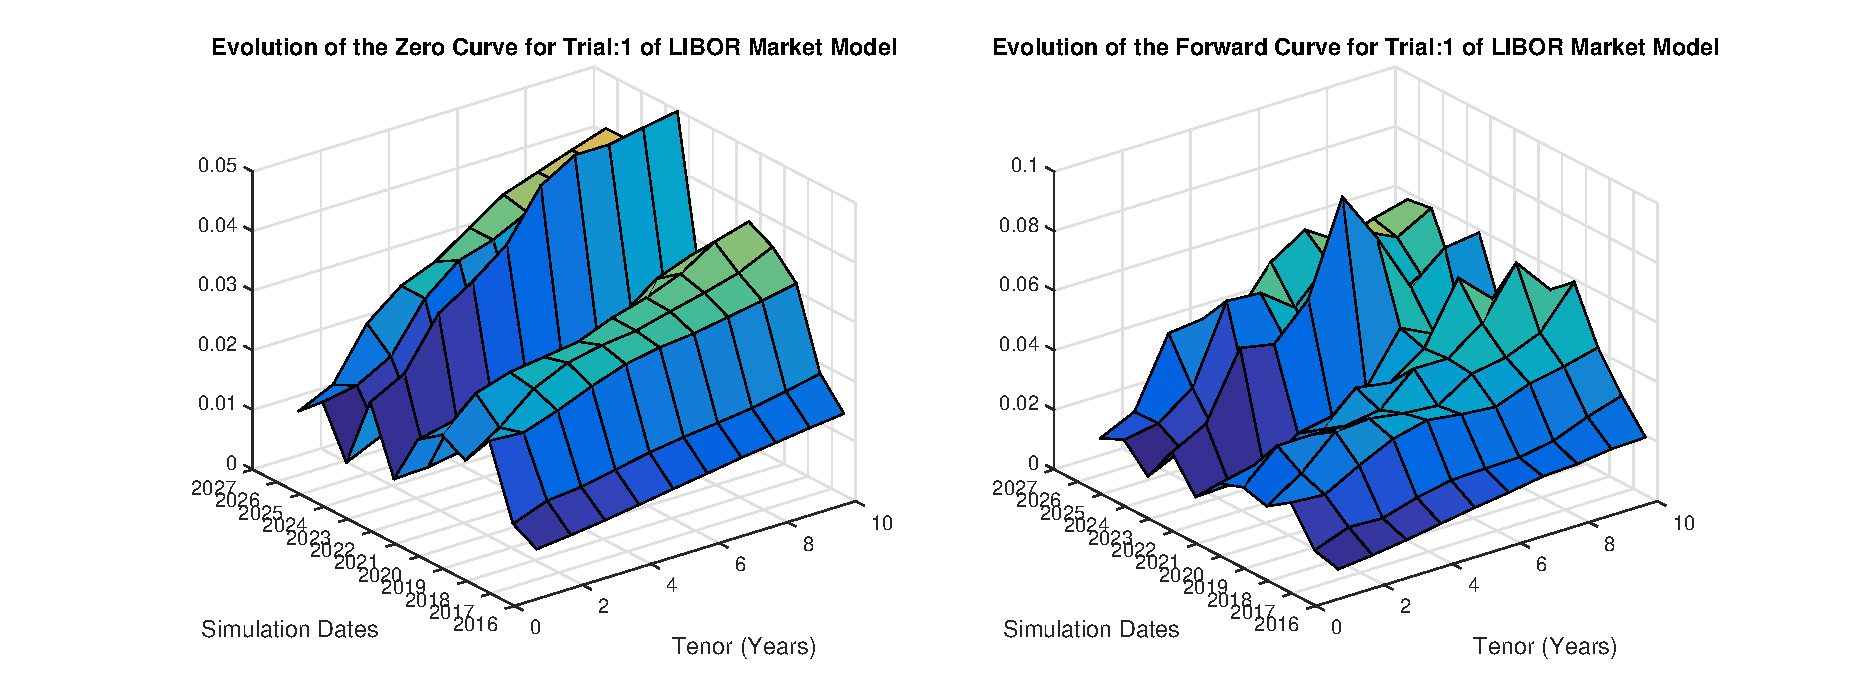
\includegraphics[scale=0.6]{sim_zero_forward.eps}
      \caption{Simulated zero curves and forward curves in one scenario from calibrated LMM.}\label{fig::sim_zero_forward}
  \end{figure}
\end{center}

\section{Price Sensitivity Analysis} \label{chpt::market_risk}
The pricing vanilla European swaption is done in the calibration process, where the Black volatility of a swaption is calculated (and compares to the market quote). A swaption price is then calculated using either Black formula for swaption or a Monte Carlo simulation using the scenarios generated from LMM. The Black formula pricing method uses the Black volatility of the swaption, which is approximated by Rebonato method. Just as an example, I price the 5-Yr-into-5-Yr (5-Yr option tenor and 5-Yr swap tenor) vanilla payer swaption with strike price 2.5\%. The fair value from the LMM is \$ 1.8236, using Monte Carlo simulation with 200 scenarios.

The market risks of this vanilla swaption are mainly {\emph Rho} and {\emph Convexity}. {\emph Rho} represents the first-order market exposure of swaption with respect to the interest rate moves. {\emph Convexity}, instead, represents the second-order market exposure of swaption with respect to the interest rate moves. The Greeks {\emph Rho} and {\emph Convexity} can be calculated from bumping the forward rate curves parallel, re-calibration on the LMM parameters, and repricing the swaption. The {\emph Rho} calculation method is
$$
Rho = \frac{\mathrm{Price when IR curve up $\Delta$ bps} - \mathrm{Price when IR curve down $\Delta$ bps}}{2\Delta}
$$

Figure~\ref{fig::swaption_prices} plots the price sensitivity of swaption with respect to the interest rate curve (OIS curve) bumpings.

\begin{center}
  \begin{figure}
      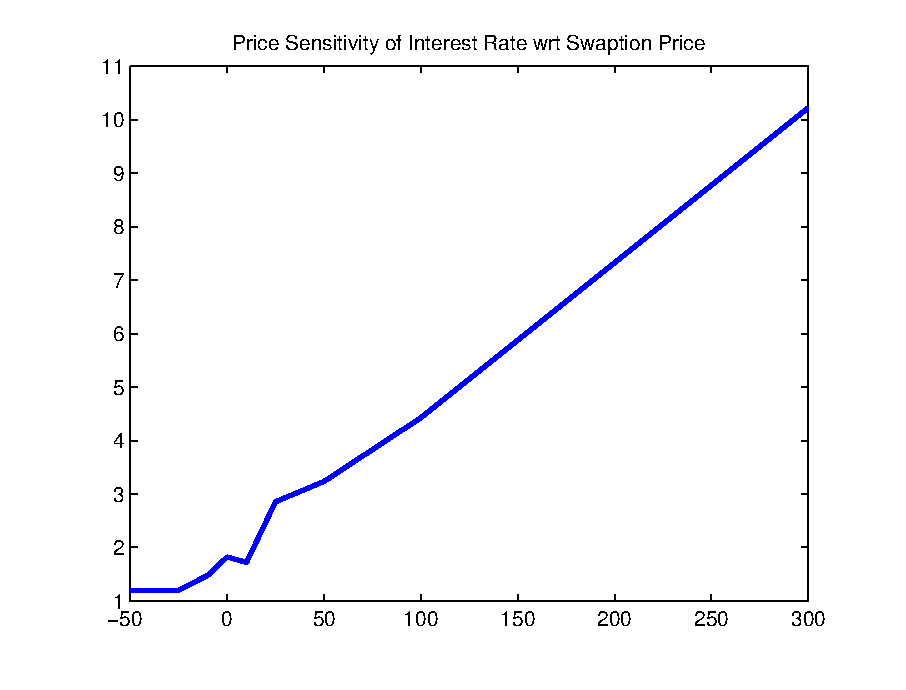
\includegraphics[scale=0.6]{swaption_prices.eps}
      \caption{The swaption prices with respect to the OIS curve bumpings.}\label{fig::swaption_prices}
  \end{figure}
\end{center}